\documentclass[titlepage, uplatex]{jsarticle}
\usepackage{h31ec-exp}
\usepackage[dvipdfmx]{graphicx}

\title{LEDの点滅回路の作成}
\grade{3年32番}
\author{平田 蓮}
\team{}
\date{2019年5月28日}
\expdate{2019年5月13日,5月20日, 5月27日}
\coauthor{}

\begin{document}
\maketitle
\section{目的}
	\begin{itemize}
		\item 電子部品に関する基礎知識や取扱方法を学ぶ.
		\item ハンダゴテやニッパなどの工具の正しい使い方を再確認する.
		\item 簡単な電子回路の動作原理を理解する.
		\item 回路図を元に基盤上での部品のレイアウトや実体配線を考える.
	\end{itemize}

\section{理論}
	図\ref{fig:LED点滅回路}は今回作成するLED点滅回路である. ~大きく分けて, ~発振回路とLED駆動回路より構成される.
	~電源に4.5[V]程度の電圧を印加すると, ~発振回路から特定周波数の矩形波が出力され, ~LED駆動回路に入力される.
	~2つのLEDはその周波数で交互に点滅を繰り返す. ~周波数は発振回路を構成する抵抗とコンデンサの値でほぼ決まる.

	\begin{figure}[h]
		\center{
			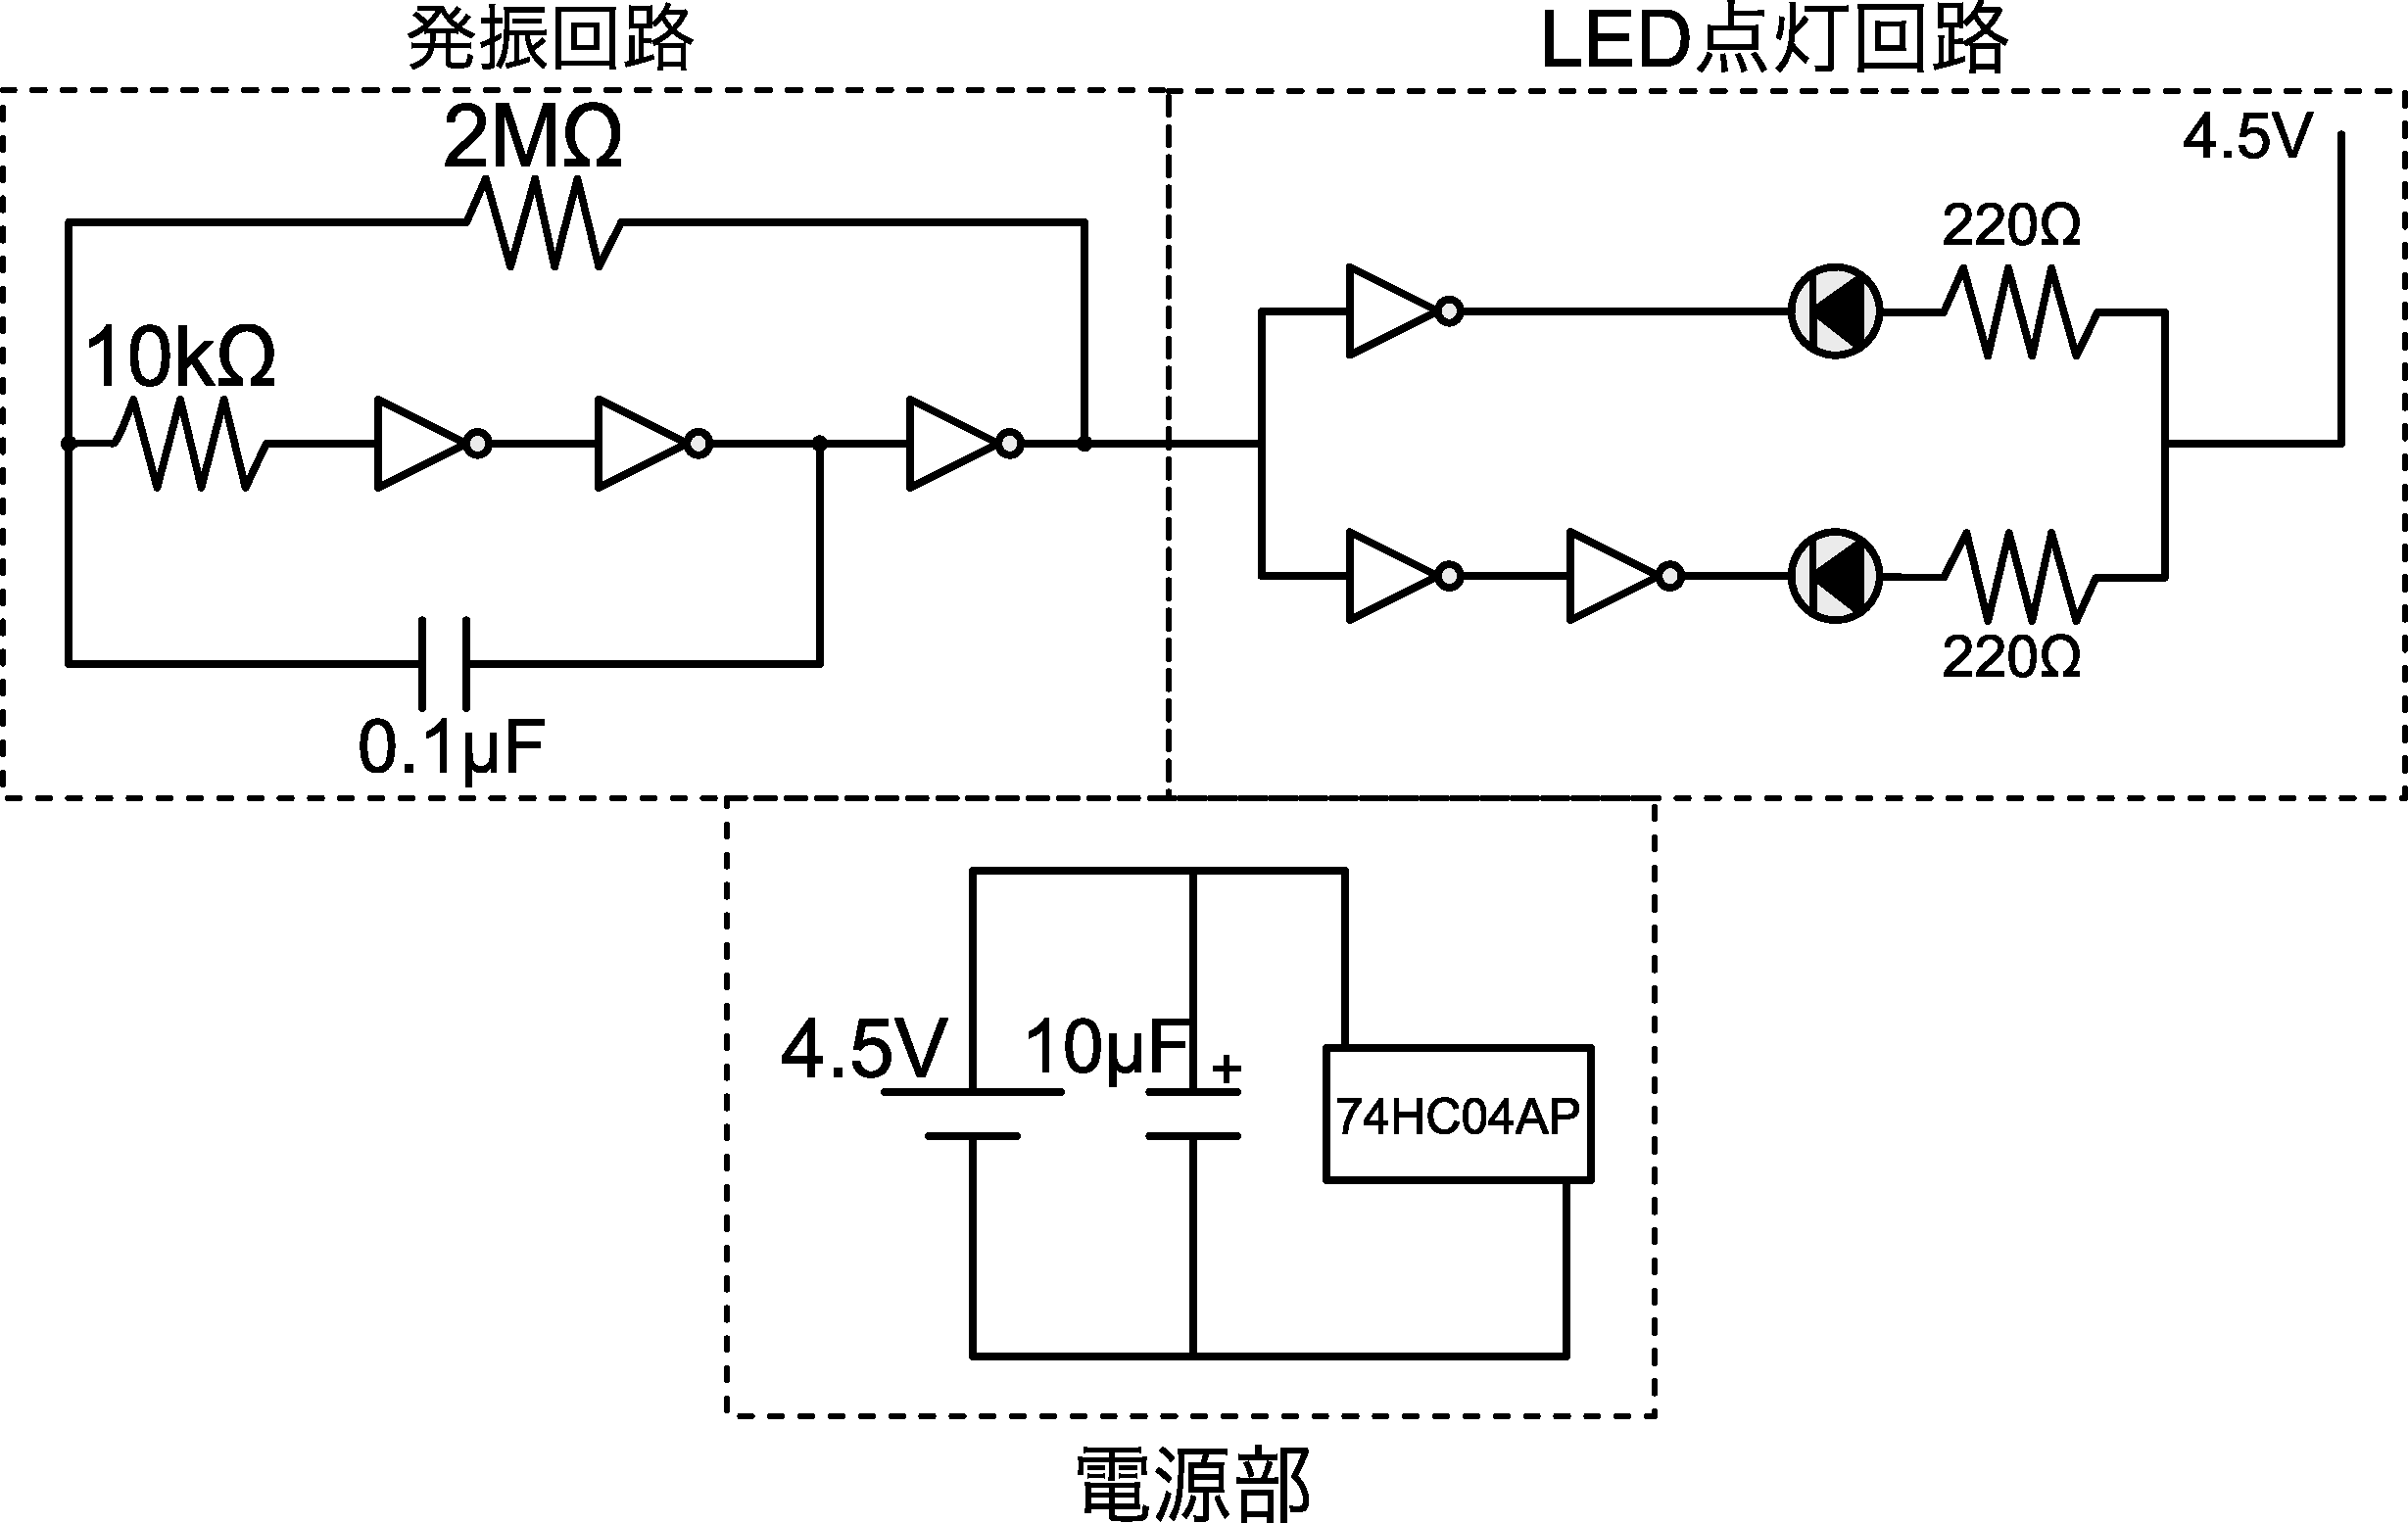
\includegraphics[width=10cm]{LED-circuit.pdf}
		}
		\caption{LED点滅回路}
		\label{fig:LED点滅回路}
	\end{figure}

	発振回路の出力部では, ~0[V]と4.5[V]の出力が交互に起こる. ~その様子を図2, ~3に示す.
	~電圧印加時は, ~図\ref{fig:説明回路1}, ~\ref{fig:説明回路2}の状態を交互に移行することで矩形波が発生する.

	\begin{figure}[h]
		\begin{tabular}{cc}
			\begin{minipage}{0.5\hsize}
				\begin{center}
					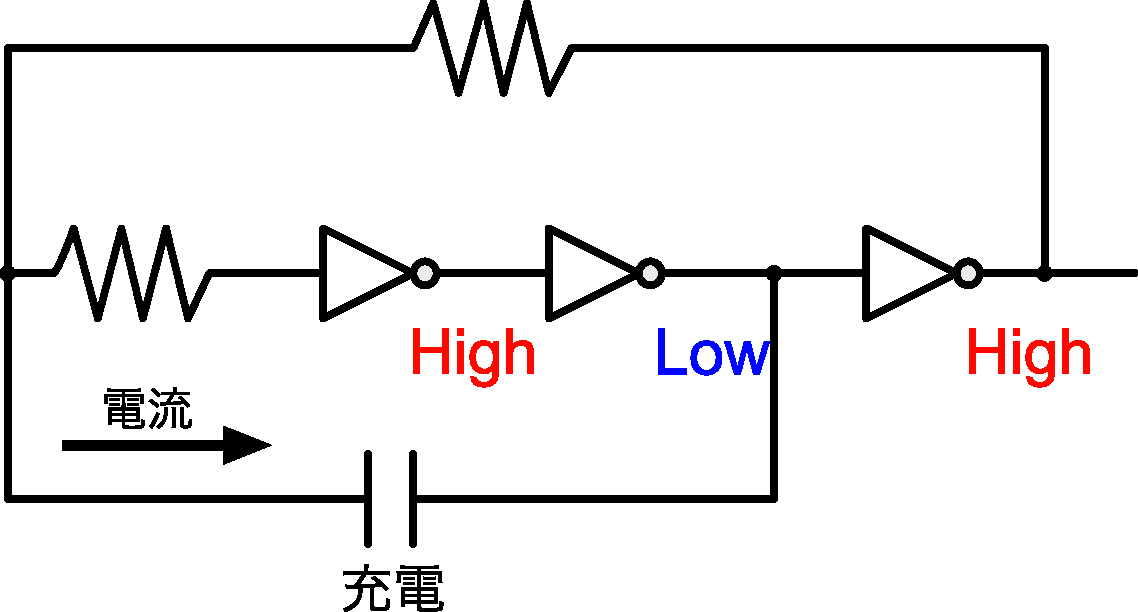
\includegraphics[width=6cm]{explain-circuit1.pdf}
				\end{center}
				\caption{動作原理1}
				\label{fig:説明回路1}
			\end{minipage}
			\begin{minipage}{0.5\hsize}
				\begin{center}
					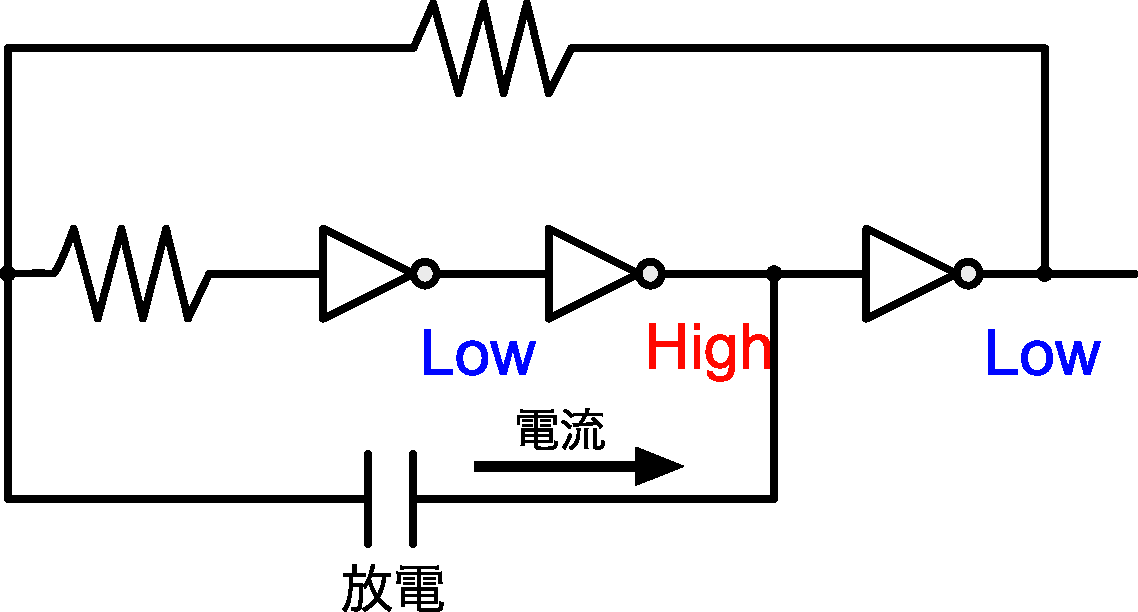
\includegraphics[width=6cm]{explain-circuit2.pdf}
				\end{center}
				\caption{動作原理2}
				\label{fig:説明回路2}
			\end{minipage}
		\end{tabular}
	\end{figure}

	ここで, ~LEDの順方向電圧を2.3[V]と仮定して, ~点灯時のLEDに流れる電流を求める.

	電源電圧を$V_{CC}$, ~LEDの順方向電圧を$V_F$とすると, ~220[$\Omega$]抵抗にかかる電圧$V_R$は,
	$$
	V_R = V_{CC} - V_F = 4.5 - 2.3 = 2.2 [\mathrm V]
	$$

	オームの法則より, ~流れる電流$I$は,
	$$
	I =\frac{V_R}{R} = \frac{2.2}{220} = 10 [\mathrm{mA}]
	$$
	と求まる.

	電源部で並列に接続されてるコンデンサは, ~電源電圧を安定させるためにある.
	~これがあることで, ~たとえICによる電流変化と電圧変化が起きても, ~足りない分の電圧をコンデンサが放電する事で補うことができる.

	~また, ~この回路の発振回路では, ~アルミ電解のコンデンサが充放電をする時間で周波数が決まっている.
	~よって, 点滅の周期を速くするには, ~アルミ電解コンデンサの静電容量を小さくするか, 2[M$\Omega$]の抵抗を小さくすれば良い.

\section{使用器具}
	\begin{itemize}
		\item はんだごて
		\item ニッパ
		\item ラジオペンチ
	\end{itemize}

\section{実験方法}
	\subsection{実体配線図の作成}
		まずはじめに, ~回路図をもとに実体配線図を作成する.
		~作成した実体配線図を図\ref{fig:実体配線図}に示す.

		\begin{figure}[h]
			\center{
				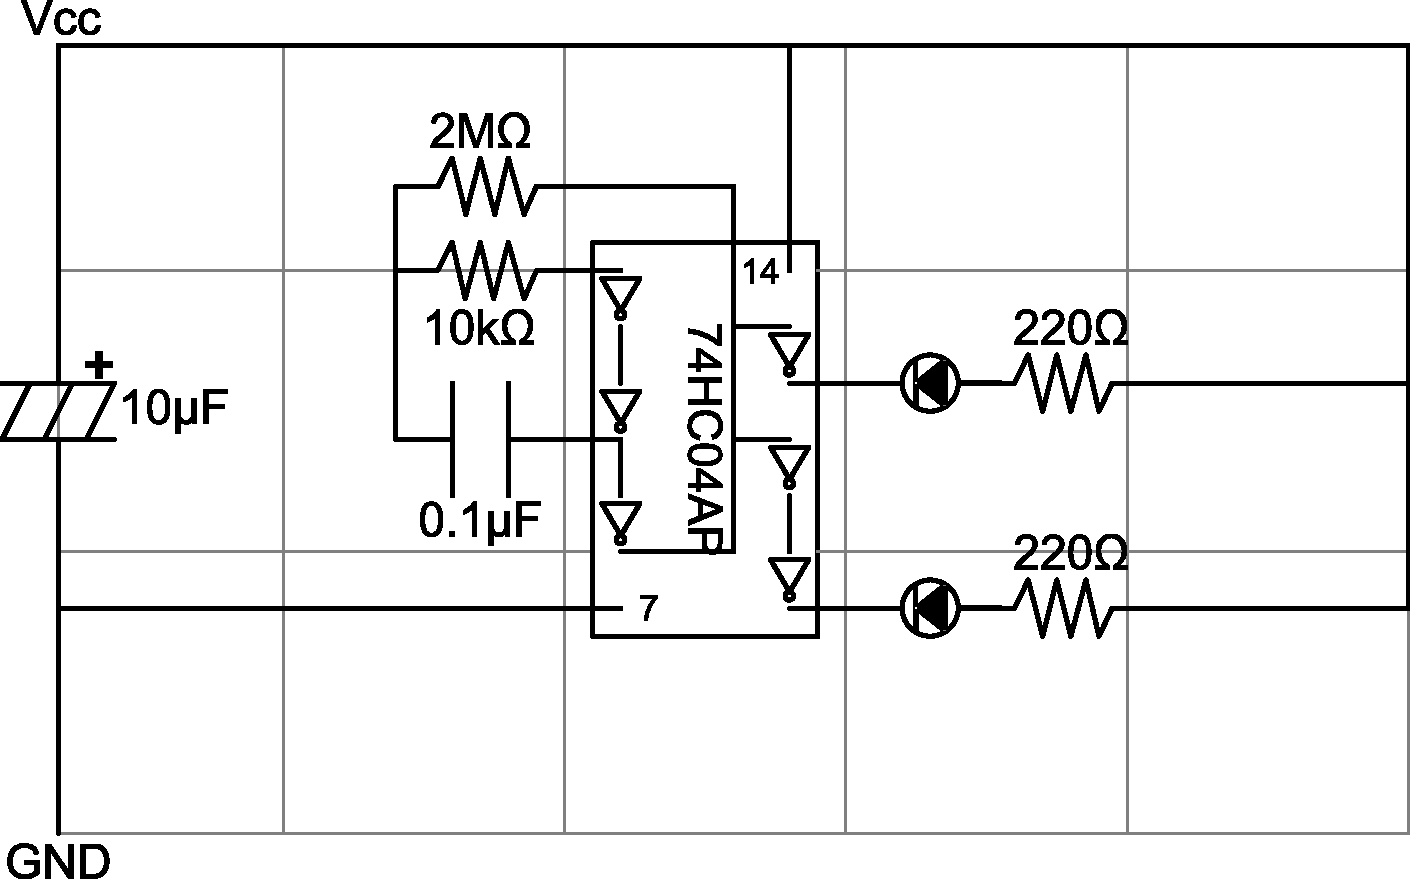
\includegraphics[width=10cm]{entity-wiring.pdf}
			}
			\caption{実体配線図}
			\label{fig:実体配線図}
		\end{figure}

		実体配線図を書く上で, ~極力配線の曲がる数を減らすようにした.
		~そうすることで組み立て時により簡単に作成することができた.

		~また, ~IC間の配線をICの裏の部分で行うことで, ~よりコンパクトな配線ができた.
		~$V_{CC}$と$GND$端子を基盤の上下端に置くことで, ~動作時にわかりやすくなるような工夫もした.

	\subsection{組み立て}
		次に実体配線図をもとに回路の組み立てを行う.
		~実体配線図は表面からみた図なので注意する.

	\subsection{動作確認}
		回路図と実体配線図をもとに, ~回路の配線に間違いがないかテスターを使ってテストする.
		~特に, ~$V_{CC}$ - $GND$間がショートしていないことを確認する.

		次に, ~回路に乾電池を直列に三つ繋いだ4.5[V]の電源を接続する.
		二つのLEDが1秒間に数回点滅していれば正しい動作である.

\section{考察}
	今回の実験を通して, ~notICを使った点滅回路を作成した.
	回路の組み立て時に, ~端子と回路がうまくつながらないことがあった.
	~そのため, ~多量のハンダを周辺で使ってしまい, ~回路の見栄えが少し悪くなってしまった.
	~これは, ~端子に使用していたリード線が, ~基盤の穴の中で切断されていて
	~うまく裏側のハンダとくっついていなかったことが考えられる.
	~この知見を次に生かしたい.

\section{感想}
	~初回の授業で実体配線図を作成した際に, ~当初は部品の配置を先に考えていたが, ~配線から考えた方がスムーズに
	書けた.実体配線図は初めて書いたが, ~回路を作成する前にこのようなことをすることをはじめて知り,
	驚いた.

	また, ~組み立て時に, ~去年の経験のおかげか, ~比較的スムーズに作業を終わらせ,
	~他の学生の手伝いをすることができた. ~その際, ~十人十色の多種多様な配線がみられて, ~興味深かった.

	次からは測定の実験なので, ~しっかりと冊子を読み込んで備えて授業に臨みたい.

\end{document}
